\documentclass[usenames,dvipsnames]{beamer}
\usepackage{xcolor}
\usepackage{tcolorbox}
\usepackage{graphicx}
\usepackage{amsmath}
\usepackage{subcaption}
\usepackage{makecell}
\usepackage[labelformat=empty]{caption}
\usepackage{color, colortbl}
\usepackage{booktabs}
\usepackage{multirow}

\usepackage{hyperref}
\hypersetup{
    colorlinks=true,
    linkcolor=blue,
    filecolor=magenta,      
    urlcolor=cyan,
}

\newcommand*{\mathcolor}{}
\def\mathcolor#1#{\mathcoloraux{#1}}
\newcommand*{\mathcoloraux}[3]{%
	\protect\leavevmode
	\begingroup
	\color#1{#2}#3%
	\endgroup
}

\usepackage{tikz}

\usetikzlibrary{shapes.geometric, arrows}
\tikzstyle{startstop} = [rectangle, rounded corners, minimum width=3cm, minimum height=1cm,text centered, draw=black, fill=brown!30]

\tikzstyle{io} = [trapezium, trapezium left angle=70, trapezium right angle=110, minimum width=3cm, minimum height=1cm, text centered, draw=black, fill=blue!30]

\def\checkmark{\tikz\fill[scale=0.4](0,.35) -- (.25,0) -- (1,.7) -- (.25,.15) -- cycle;} 

\tikzstyle{arrow} = [thick,->,>=stealth]


\newcommand{\DoTikzmark}[1]{%
	\tikz[remember picture] \coordinate[shift={(0,.7ex)}](#1);%
}

\newcommand{\colrow}[3][]{%
	\tikz[overlay,remember picture, line width=10pt]
	\draw[shorten >=-.1em, shorten <=-.1em, #1] (#2)--(#3);
}


\newcolumntype{g}{>{\columncolor{Lavender}}c}
\newcolumntype{t}{>{\columncolor{Tan}}c}

%\beamerdefaultoverlayspecification{<+->}
\newcommand{\data}{\mathcal{D}}

\DeclareMathOperator*{\argmin}{arg\,min}

\newcommand\Item[1][]{%
	\ifx\relax#1\relax  \item \else \item[#1] \fi
	\abovedisplayskip=0pt\abovedisplayshortskip=0pt~\vspace*{-\baselineskip}}
	


\usetheme{metropolis}           % Use metropolis theme


\title{Convention, Accuracy metrics, Classification, Regression}
\date{\today}
\author{Nipun Batra}
\institute{IIT Gandhinagar}
\begin{document}
  \maketitle
  
  
  
\begin{frame}{Logistics}
\begin{itemize}
	\item \pause Please sign up on Google Classroom: {\Huge cgt6rwd}
	\item \pause Extra lecture on Saturday, 11 Jan at 11 AM in 1/101
	\item \pause FAQ, Project google docs open for comments. Please use comments to seek clarity.
	\item \pause Video and slides from last lecture up on course website: https://sites.google.com/view/es654-2020/
\end{itemize}
\end{frame}

\begin{frame}{Revision: What is Machine Learning}

	\pause``Field of study that give computers the ability to learn
	without being explicitly programmed'' - Arthur Samuel
	[1959]
	\vspace{-10pt}
	\pause \begin{figure}
		\centering
		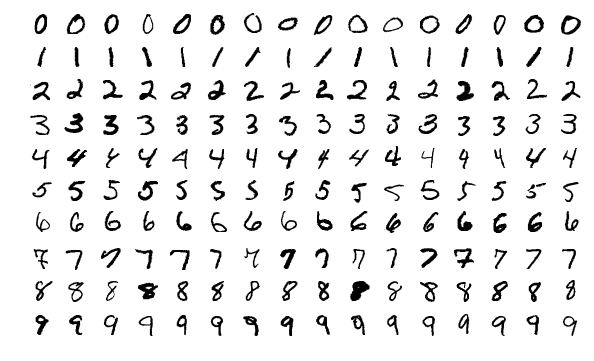
\includegraphics[width=0.25\linewidth]{mnist}
		\caption{}\vspace{-20pt}
		\label{fig:mnist}
	\end{figure}
	\vspace{-20pt}
	\pause How would you program to recognise digits? Start with 4.
	
	\pause Maybe 4 can be thought of as: ``|'' + ``\_\_''  + ``|'' + another vertically down ``|''
	
	\pause The heights of each of the ``|'' need to be similar within tolerance
	
	\pause Each of the ``|'' can be slightly slanted. Similarly the horizontal line can be slanted.
	\pause There can be some cases of 4 where the first ``|'' is at 45 degrees
	\pause There can be some cases of 4 where the width of each stroke is different
	


\end{frame}	



\begin{frame}

\begin{tikzpicture}[node distance=2cm]
\node (Data) [startstop] {Data};
\node (Rules) [startstop, below of=Data] {Rules};
\node (Traditional) [startstop, right of=Data, xshift=2cm, yshift=-1cm] {\makecell[l]{Traditional\\Programming}};
\node (Answers) [startstop, right of=Traditional, xshift=2cm] {Answers};
\draw [arrow] (Data) -- (Traditional);
\draw [arrow] (Rules) -- (Traditional);
\draw [arrow] (Traditional) -- (Answers);
\end{tikzpicture}
\vspace{40pt}

\pause \begin{tikzpicture}[node distance=2cm]
\node (Data) [startstop] {Data};
\node (Answers) [startstop, below of=Data] {Answers};
\node (ML) [startstop, right of=Data, xshift=2cm, yshift=-1cm] {\makecell[l]{Machine \\Learning}};
\node (Rules) [startstop, right of=ML, xshift=2cm] {Rules};
\draw [arrow] (Data) -- (ML);
\draw [arrow] (Answers) -- (ML);
\draw [arrow] (ML) -- (Rules);
\end{tikzpicture}
	
\end{frame}

\begin{frame}{Revision: What is Machine Learning}
``A computer program is said to learn from
experience E with respect to some class of tasks T
and performance measure P if its performance at
tasks in T, as measured by P, improves with
experience E.'' - Tom Mitchell
\end{frame}

\begin{frame}{First ML Task: Grocery store tomatoes quality prediction}
Problem statement: You want to predict the quality/condition of a tomato given its visual features.
\end{frame}

\begin{frame}{Dataset}
Imagine you have some past data on quality of tomatoes. What visual features do you think will be useful?

\begin{itemize}
	\item \pause Size
	\item \pause Colour
	\item \pause Texture
\end{itemize}
\end{frame}
  
\begin{frame}{Dataset}
Imagine you have some past data on quality of tomatoes. 

\begin{table}[]
	\begin{tabular}{|l|l|l|l||l|}
		\hline 
		\textbf{Sample} & \textbf{Colour} & \textbf{Size} & \textbf{Texture} & \textbf{Condition} \\ \hline 
		1      & Orange & Small & Smooth  & Good      \\
		2      & Red    & Small  & Rough  & Good \\
		3      & Orange & Medium & Smooth & Bad \\
		4      & Yellow & Large  & Smooth & Bad \\ \hline          
	\end{tabular}
\end{table}
\end{frame}

\begin{frame}{Useful Features}
Is the sample number a useful feature for predicting quality of a tomato?

\pause Answer: It depends! Maybe, all tomatoes received after a certain date are bad! Let us ignore that for now.

\pause Let us modify our data table for now.

\begin{table}[]
	\begin{tabular}{|l|l|l||l|}
		\hline 
		\textbf{Colour} & \textbf{Size} & \textbf{Texture} & \textbf{Condition} \\ \hline 
		Orange & Small & Smooth  & Good      \\
		Red    & Small  & Rough  & Good \\
		Orange & Medium & Smooth & Bad \\
		Yellow & Large  & Smooth & Bad \\ \hline 

	\end{tabular}
\end{table}
\end{frame}

\begin{frame}{Training Set}

\begin{table}[]
	\begin{tabular}{|g|g|g||t|}
		\hline 
				\rowcolor{white}
		\textbf{Colour} & \textbf{Size} & \textbf{Texture} & \textbf{Condition} \\ \hline 
		Orange & Small & Smooth  & Good      \\
		Red    & Small  & Rough  & Good \\
		Orange & Medium & Smooth & Bad \\
		Yellow & Large  & Smooth & Bad \\ \hline 
		
	\end{tabular}
\end{table}

\pause The training set consists of two parts:
\begin{enumerate}
	\item \pause \color{Lavender}{Features, Attributes or Covariates}
	\item \pause \color{Tan}{Output or Response Variable}
\end{enumerate}
\end{frame}

\begin{frame}{Training Set}
\vspace{-5pt}
\begin{table}[]
	\begin{tabular}{|g|g|g||t|}
		\hline 
		\rowcolor{white}
		\textbf{Colour} & \textbf{Size} & \textbf{Texture} & \textbf{Condition} \\ \hline 
		Orange & Small & Smooth  & Good      \\
		Red    & Small  & Rough  & Good \\
		Orange & Medium & Smooth & Bad \\
		Yellow & Large  & Smooth & Bad \\ \hline 
		
	\end{tabular}
\end{table}


\pause We call this matrix as $\mathcal{D}$, containing:
\begin{enumerate}
	\item \pause Feature matrix ($\mathbf{X \in \mathcal{R}^{N\times P}}$) containing data of $N$ samples each of which is $P$ dimensional.
	\begin{itemize}
		\item \pause Thus, $\mathbf{X} = \{x_i^T\}_{i=1}^N$ where $x_i \in \mathcal{R}^P$
		\item \pause Example $x_1 = \begin{bmatrix}
		Orange \\
		Small \\
		Smooth \\
		\end{bmatrix}
		$
	\end{itemize}
\item \pause Output Vector ($y \in \mathcal{R}^N$) containing output variable for $N$ samples.
\item \pause Thus, we can also write $\mathcal{D} = \{(x_i^T, y_i)\}_{i=1}^N$
\end{enumerate}

\end{frame}


\begin{frame}{Prediction Task}
Estimate condition for unseen tomatoes (\#5, 6) based on data set. 

\begin{table}[]
	\begin{tabular}{|l|l|l||l|}
		\hline 
		
		\textbf{Colour} & \textbf{Size} & \textbf{Texture} & \textbf{Condition} \\ \hline 
		Orange & Small & Smooth  & Good      \\
		Red    & Small  & Rough  & Good \\
		Orange & Medium & Smooth & Bad \\
		Yellow & Large  & Smooth & Bad \\ \hline
		Red    & Large  & Rough  & ? \\
		Orange &  Large & Rough  & ? \\ \hline          
	\end{tabular}
\end{table}
\end{frame}

\begin{frame}{Testing Set}
\textcolor{YellowGreen}{Testing set} is similar to \textcolor{Peach}{training set}, but, does not contain labels for output variable. 

\begin{table}[]
	\begin{tabular}{|l|l|l||l|}
		\hline 
		\textbf{Colour} & \textbf{Size} & \textbf{Texture} & \textbf{Condition} \\ \hline 
		\rowcolor{Peach}
		Orange & Small & Smooth  & Good      \\
		\rowcolor{Peach}
		Red    & Small  & Rough  & Good \\
		\rowcolor{Peach}
		Orange & Medium & Smooth & Bad \\
		\rowcolor{Peach}
		Yellow & Large  & Smooth & Bad \\ \hline
				\rowcolor{YellowGreen}
		Red    & Large  & Rough  & ? \\
		\rowcolor{YellowGreen}
		Orange &  Large & Rough  & ? \\ \hline          
	\end{tabular}
\end{table}
\end{frame}



\begin{frame}{Prediction Task}
We hope to:
\begin{enumerate}
	\item \pause Learn $f$: 		$\text{Condition} = f(\text{colour, size, texture})$
	\item \pause From Training Dataset
	\item \pause To Predict the condition for the Testing set
\end{enumerate}


\begin{table}[]
	\begin{tabular}{|l|l|l||l|}
		\hline 
		
		\textbf{Colour} & \textbf{Size} & \textbf{Texture} & \textbf{Condition} \\ \hline 
		Orange & Small & Smooth  & Good      \\
		Red    & Small  & Rough  & Good \\
		Orange & Medium & Smooth & Bad \\
		Yellow & Large  & Smooth & Bad \\ \hline
		Red    & Large  & Rough  & ? \\
		Orange &  Large & Rough  & ? \\ \hline          
	\end{tabular}
\end{table}
\end{frame}

\begin{frame}{Generalisation}
\begin{itemize}
	\item Q: Is predicting on test set enough to say our model generalises? 
	\item \pause A: Ideally, no!
	\item \pause Ideally - we want to predict ``well'' on all possible inputs. But, can we test that?
	\item \pause No! Since, the test set is only a sample from all possible inputs.
\end{itemize}





\end{frame}

\begin{frame}{Generalisation}
\begin{figure}
	\centering
	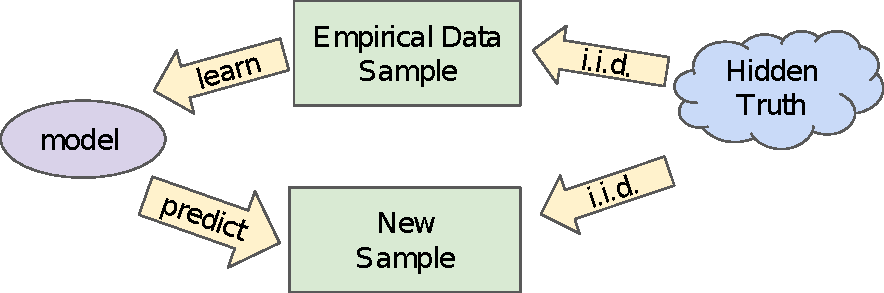
\includegraphics[width=0.8\textwidth]{train-test}
	\caption{Image courtesy Google ML crash course}
	\label{fig:train-test}
\end{figure}

\pause Both the training set and the test set are samples drawn from the hidden true distribution (also sometimes called population)

\pause More discussion later once we study bias and variance
\end{frame}

\begin{frame}{Second ML Task: Predict energy consumption of campus}

Question: What factors does the campus energy consumption depend on?

Answer:\begin{itemize}
	\item \pause \# People (More people $\implies$ More Energy)
	\item \pause Temperature (Higher Temp. $\implies$ Higher Energy)

\pause \begin{table}[]
	\begin{tabular}{|l|l||l|}
		\hline 
		
		\textbf{\# People} & \textbf{Temp (C)} &  \textbf{Energy (kWh)} \\ \hline 
		
		4000 & 30 & 30 \\
		4200 & 30 & 32 \\
		4200 & 35 & 40 \\ \hline
		3000 & 20& ? \\
		1000 & 45 & ? \\ \hline          
	\end{tabular}
\end{table}	
\end{itemize}

\end{frame}





\begin{frame}{Classification v/s Regression}
\begin{itemize}
	\item Classification
	\begin{itemize}
		\item \pause Output variable is discrete
		\item \pause i.e.  $y_i\in \{1, \cdots C\}$ 
		\item \pause Examples - Predicting: 
		\begin{itemize}
			\item \pause Will I get a loan? (Yes, No)
			\item \pause What is the quality of fruit? (Good, Bad)
		\end{itemize}
	\end{itemize}
	\item \pause Regression
	\begin{itemize}
		\item \pause Output variable is continuous
		\item \pause i.e.  $y_i\in \mathcal{R}$ 
		\item \pause Examples - Predicting: 
		\begin{itemize}
			\item \pause How much energy will campus consume? 
			\item \pause How much rainfall will fall?
		\end{itemize}
	\end{itemize}
\end{itemize}

\end{frame}

%\begin{frame}{Feature Table}
%\begin{figure}[htp]
%    \centering
%    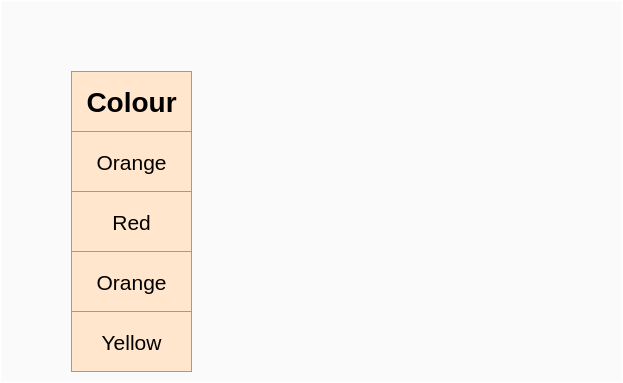
\includegraphics[width=0.7\linewidth]{accuracy/ml_2_accuracy_table_1.png}
%\end{figure}
%\end{frame}

%\captionsetup[subtable]{labelformat=empty}
%
%\begin{frame}{Metrics for Classification}
%\begin{table}[!htb]
%	\caption{}
%	\begin{subtable}{.5\linewidth}
%		\centering
%		\caption{Prediction ($\hat{y}$)}
%		\begin{tabular}{ |c| } \hline 
%			
%			Good \\
%			Good \\
%			Good \\
%			Good \\
%			Bad  \\ \hline 
%			
%		\end{tabular}
%	\end{subtable}%
%	\begin{subtable}{.5\linewidth}
%		\centering
%		\caption{Ground Truth ($y$)}
%		\begin{tabular}{ |c| } 
%			\hline 
%			Good \\
%			Good \\
%			Bad \\
%			Bad  \\
%			Bad \\ \hline 
%		\end{tabular} \\
%	\end{subtable} 
%\end{table}
%
%\begin{align*}
%\text{Accuracy} &= \frac{||y = \hat{y}||}{||y||} \end{align*}
%\end{frame}

%\begin{frame}{Metrics for Classification}
%\begin{table}[!htb]
%	\caption{}
%	\begin{subtable}{.5\linewidth}
%		\centering
%		\caption{Prediction ($\hat{y}$)}
%		\begin{tabular}{ |c| } \hline 
%			
%			\rowcolor{Green}Good \\
%			\rowcolor{Green}Good \\
%			\rowcolor{Red}Good \\
%			\rowcolor{Red}Good \\
%			\rowcolor{Green}Bad  \\ \hline 
%			
%		\end{tabular}
%	\end{subtable}%
%	\begin{subtable}{.5\linewidth}
%		\centering
%		\caption{Ground Truth ($y$)}
%		\begin{tabular}{ |c| } 
%			\hline 
%			Good \\
%			Good \\
%			Bad \\
%			Bad  \\
%			Bad \\ \hline 
%		\end{tabular} \\
%	\end{subtable} 
%\end{table}
%
%\begin{align*}
%\text{Accuracy} &= \frac{||y = \hat{y}||}{||y||} \\
%&= \frac{3}{5} = 0.6
%\end{align*}
%\end{frame}
%
%%\begin{frame}
%%\setlength{\tabcolsep}{12pt}
%%\begin{tabular}{ cc }   % top level tables, with 2 rows
%%	Ground Truth ($y$) & Prediction ($\hat{y}$) \\  
%%	% bottom left of the top level table: table 1 
%%	\begin{tabular}{ |c| } 
%%		
%%		Good \\
%%		Good \\
%%		Good \\
%%		Good \\
%%		Bad  \\
%%		
%%	\end{tabular} &  % starting bottom right of the top level table
%%	% table 2
%%	\begin{tabular}{ |c| } 
%%		Good \\
%%		Good \\
%%		Bad \\
%%		Bad  \\
%%		Bad \\
%%	\end{tabular} \\
%%\end{tabular}
%%\end{frame}
%%
%%\begin{frame}{Metrics for Classification}
%%
%%
%%
%%$
%%Prediction (\hat{y}) = \begin{bmatrix}
%%	Good \\
%%	Good \\
%%	Good \\
%%	Good \\
%%	Bad  \\
%%\end{bmatrix} ~~~~Ground Truth (y) = \begin{bmatrix}
%%Good \\
%%Good \\
%%Bad \\
%%Bad  \\
%%Bad \\
%%\end{bmatrix}$ 
%%\vspace{30pt}
%%
%%\begin{itemize}
%%	\item Ground Truth: From the actual training set 
%%	\item Prediction: Made by the model
%%\end{itemize}
%%
%%\end{frame}
%%
%%\begin{frame}{Metrics for Classification}
%%%\DoTikzmark{num-3}{-}3 & 0 & {4}\DoTikzmark{num4}
%%$
%%Prediction (\hat{y}) = \begin{bmatrix}
%%Good \\
%%Good \\
%%Good \\
%%Good \\
%%Bad  \\
%%\end{bmatrix} ~~~~Ground Truth (y) = \begin{bmatrix}
%%Good \\
%%Good \\
%%Bad \\
%%Bad  \\
%%Bad \\
%%\end{bmatrix}$ 
%%
%%
%%\vspace{30pt}
%
%
%
%%\end{frame}



\begin{frame}{Metrics for Classification}



$$\bordermatrix{&\text{Prediction}\;(\hat{y})\cr
                &\text{Good}\cr
                &\text{Good}\cr
                &\text{Good}\cr
                &\text{Good}\cr
                &\text{Bad}}
                \qquad \qquad
   \bordermatrix{&\text{Ground Truth}\;(y)\cr
                &\text{Good}\cr
                &\text{Good}\cr
                &\text{Bad}\cr
                &\text{Bad}\cr
                &\text{Bad}}
$$

\vspace{1cm}

\begin{tabular}{ll}
Ground Truth: & From the actual training set \\ 
Prediction: & Made by the model \\ 
\end{tabular}

\end{frame}

\begin{frame}{Accuracy}
$$
\bordermatrix{&\text{Prediction}\;(\hat{y})\cr
               \checkmark&\text{Good}\cr
               \checkmark&\text{Good}\cr
                &\text{Good}\cr
                &\text{Good}\cr
               \checkmark&\text{Bad}}
\qquad \qquad
\bordermatrix{&\text{Ground Truth}\;(y)\cr
                &\text{Good}\cr
                &\text{Good}\cr
                &\text{Bad}\cr
                &\text{Bad}\cr
                &\text{Bad}}
$$

\pause \begin{align*}
\text{Accuracy} &= \frac{||y = \hat{y}||}{||y||} \\ 
&= \frac{3}{5} = 0.6
\end{align*}

\end{frame}

\begin{frame}{Types of Data: Imbalanced Classes}
\[
  \begin{array}{@{} c @{}}
    \begin{array}{@{} r @{}}
      \text{1 sample}~\{\hspace{\nulldelimiterspace} \\
      \text{100 samples}~\left\{\begin{array}{@{}c@{}}\null\\\null\\\null\\\null\end{array}\right.
    \end{array}
    \left (
      \begin{array}{ *{1}{c} }
        \text{Bad}  \\
        \text{Good}  \\
        \text{Good}  \\
        \ldots  \\
        \text{Good}  \\
      \end{array}
    \right ) \\
    \mathstrut
  \end{array}
  \quad \quad \quad
  \text{Imbalanced Classes}
\]

\pause

Cases for this:
\begin{itemize}%[<+->]
\item Cancer Screening
\item Planet Detection
\end{itemize}

\end{frame}

\begin{frame}{Accuracy Metrics: Precision}
$$
\bordermatrix{&\text{Prediction}\;(\hat{y})\cr
               \rightarrow\checkmark&\text{Good}\cr
               \rightarrow\checkmark&\text{Good}\cr
                \rightarrow&\text{Good}\cr
                \rightarrow&\text{Good}\cr
               &\text{Bad}}
\qquad \qquad
\bordermatrix{&\text{Ground Truth}\;(y)\cr
                &\text{Good}\cr
                &\text{Good}\cr
                &\text{Bad}\cr
                &\text{Bad}\cr
                &\text{Good}}
$$

\begin{align*}
\pause \text{Precision} &= \frac{||y = \hat{y} = \text{Good}||}{||\hat{y} = \text{Good}||} = \frac{2}{4} = 0.5
\end{align*}

``the fraction of relevant instances among the retrieved instances'', i.e. ``out of the number of times we predict \text{Good}, how many times is the condition actually \text{Good}''

\end{frame}

\begin{frame}{Accuracy Metrics: Recall}
$$
\bordermatrix{&\text{Prediction}\;(\hat{y})\cr
               \rightarrow\checkmark&\text{Good}\cr
               \rightarrow\checkmark&\text{Good}\cr
                &\text{Good}\cr
                &\text{Good}\cr
               \rightarrow&\text{Bad}}
\qquad \qquad
\bordermatrix{&\text{Ground Truth}\;(y)\cr
                &\text{Good}\cr
                &\text{Good}\cr
                &\text{Bad}\cr
                &\text{Bad}\cr
                &\text{Good}}
$$

\begin{align*}
\text{Recall} &= \frac{||y = \hat{y} = \text{Good}||}{||y = \text{Good}||} = \frac{2}{3} = 0.67
\end{align*}

``the fraction of the total amount of relevant instances that were actually retrieved''

\end{frame}

\begin{frame}{Types of Data: Imbalanced Classes}
Given predictions of whether a tissue is cancerous or not ($n = 100$).
$$
\bordermatrix{&\text{Prediction}\;(\hat{y})\cr
               \rightarrow&\text{Yes}\cr
               &\text{No}\cr
                &\text{No}\cr
                &\ldots\cr
               &\text{No}}
\qquad \qquad
\bordermatrix{&\text{Ground Truth}\;(y)\cr
                &\text{No}\cr
                &\text{No}\cr
                &\ldots\cr
                &\text{No}\cr
                \rightarrow&\text{Yes}}a
            $$

\pause 
\begin{align*}
\text{Accuracy} = \frac{98}{100} = 0.98 \qquad \qquad \qquad
\text{Recall} &= \frac{0}{1} = 0 \\
\text{Precision} &= \frac{0}{1} = 0
\end{align*}


\end{frame}

\begin{frame}{Accuracy Metrics: Confusion Matrix}
\begin{center}


\begin{tabular}{@{}cc cc@{}}
	\multicolumn{1}{c}{} &\multicolumn{1}{c}{} &\multicolumn{2}{c}{Ground Truth} \\ 
	\cmidrule(lr){3-4}
	\multicolumn{1}{c}{} & 
	\multicolumn{1}{c}{} & 
	\multicolumn{1}{c}{Yes} & 
	\multicolumn{1}{c}{No} \\ 
	\cline{2-4}
	\multirow[c]{2}{*}{\rotatebox[origin=tr]{90}{Predicted}}
	& Yes  & 0 & 1   \\[1.5ex]
	& No  & 1   & 98 \\ 
	\cline{2-4}
\end{tabular}

\pause 
\vspace{60pt}
\begin{tabular}{@{}cc cc@{}}
	\multicolumn{1}{c}{} &\multicolumn{1}{c}{} &\multicolumn{2}{c}{Ground Truth} \\ 
	\cmidrule(lr){3-4}
	\multicolumn{1}{c}{} & 
	\multicolumn{1}{c}{} & 
	\multicolumn{1}{c}{Yes} & 
	\multicolumn{1}{c}{No} \\ 
	\cline{2-4}
	\multirow[c]{2}{*}{\rotatebox[origin=tr]{90}{Predicted}}
	& Yes  & True Positive & False Positive   \\[1.5ex]
	& No  & False Negative   & True Negative \\ 
	\cline{2-4}
\end{tabular}
\end{center}
\end{frame}

\begin{frame}{Accuracy Metric: Confusion Matrix}
\begin{center}
	\begin{tabular}{@{}cc cc@{}}
		\multicolumn{1}{c}{} &\multicolumn{1}{c}{} &\multicolumn{2}{c}{Ground Truth} \\ 
		\cmidrule(lr){3-4}
		\multicolumn{1}{c}{} & 
		\multicolumn{1}{c}{} & 
		\multicolumn{1}{c}{Yes} & 
		\multicolumn{1}{c}{No} \\ 
		\cline{2-4}
		\multirow[c]{2}{*}{\rotatebox[origin=tr]{90}{Predicted}}
		
		& Yes  & \cellcolor{blue!25}True Positive & \cellcolor{blue!25}False Positive   \\[1.5ex]
		& No  & False Negative   & True Negative \\ 
		\cline{2-4}
	\end{tabular}\\
	
	\vspace{30pt}
	Precision = $\frac{T.P.}{T.P. + F.P.}$
\end{center}
\end{frame}

\begin{frame}{Accuracy Metric: Confusion Matrix}
\begin{center}
\begin{tabular}{@{}cc cc@{}}
	\multicolumn{1}{c}{} &\multicolumn{1}{c}{} &\multicolumn{2}{c}{Ground Truth} \\ 
	\cmidrule(lr){3-4}
	\multicolumn{1}{c}{} & 
	\multicolumn{1}{c}{} & 
	\multicolumn{1}{c}{Yes} & 
	\multicolumn{1}{c}{No} \\ 
	\cline{2-4}
	\multirow[c]{2}{*}{\rotatebox[origin=tr]{90}{Predicted}}
	
	& Yes  & \cellcolor{blue!60}True Positive & \cellcolor{blue!25}False Positive   \\[1.5ex]
	& No  & False Negative   & True Negative \\ 
	\cline{2-4}
\end{tabular}\\

\vspace{30pt}
Precision = $\frac{T.P.}{T.P. + F.P.}$
\end{center}
\end{frame}

\begin{frame}{Accuracy Metric: Confusion Matrix}
\begin{center}
	\begin{tabular}{@{}cc cc@{}}
		\multicolumn{1}{c}{} &\multicolumn{1}{c}{} &\multicolumn{2}{c}{Ground Truth} \\ 
		\cmidrule(lr){3-4}
		\multicolumn{1}{c}{} & 
		\multicolumn{1}{c}{} & 
		\multicolumn{1}{c}{Yes} & 
		\multicolumn{1}{c}{No} \\ 
		\cline{2-4}
		\multirow[c]{2}{*}{\rotatebox[origin=tr]{90}{Predicted}}
		
		& Yes  & \cellcolor{blue!25}True Positive &False Positive   \\[1.5ex]
		& No  &  \cellcolor{blue!25}False Negative   & True Negative \\ 
		\cline{2-4}
	\end{tabular}\\
	
	\vspace{30pt}
	Recall = $\frac{T.P.}{T.P. + F.N.}$
\end{center}
\end{frame}

\begin{frame}{Accuracy Metric: Confusion Matrix}
\begin{center}
	\begin{tabular}{@{}cc cc@{}}
		\multicolumn{1}{c}{} &\multicolumn{1}{c}{} &\multicolumn{2}{c}{Ground Truth} \\ 
		\cmidrule(lr){3-4}
		\multicolumn{1}{c}{} & 
		\multicolumn{1}{c}{} & 
		\multicolumn{1}{c}{Yes} & 
		\multicolumn{1}{c}{No} \\ 
		\cline{2-4}
		\multirow[c]{2}{*}{\rotatebox[origin=tr]{90}{Predicted}}
		
		& Yes  & \cellcolor{blue!50}True Positive &False Positive   \\[1.5ex]
		& No  &  \cellcolor{blue!25}False Negative   & True Negative \\ 
		\cline{2-4}
	\end{tabular}\\
	
	\vspace{30pt}
	Recall = $\frac{T.P.}{T.P. + F.N.}$
\end{center}
\end{frame}


%\begin{frame}{Accuracy Metrics: Confusion Matrix}
%For the same data
%\pause $$
%\bordermatrix{&\text{G.T. Positive}&\text{G.T. Negative}\cr
%               \text{Pred Positive}&0&1\cr
%               \text{Pred Negative}&1&98}
%$$
%\pause $$
%\bordermatrix{&\text{G.T. Positive}&\text{G.T. Negative}\cr
%               \text{Pred Positive}&\text{True Positive}&\text{False Positive}\cr
%               \text{Pred Negative}&\text{True Negative}&\text{False Negative}}
%$$
%
%
%\pause \begin{align*}
%\text{Recall} = \frac{\text{T.P}}{\text{T.P + F.P}} \qquad \qquad 
%\text{Precision} = \frac{\text{T.P}}{\text{T.P + F.N}}
%\end{align*}
%\end{frame}

\begin{frame}{Accuracy Metrics: F-Score}

\begin{center}
	\begin{tabular}{@{}cc cc@{}}
		\multicolumn{1}{c}{} &\multicolumn{1}{c}{} &\multicolumn{2}{c}{Ground Truth} \\ 
		\cmidrule(lr){3-4}
		\multicolumn{1}{c}{} & 
		\multicolumn{1}{c}{} & 
		\multicolumn{1}{c}{Yes} & 
		\multicolumn{1}{c}{No} \\ 
		\cline{2-4}
		\multirow[c]{2}{*}{\rotatebox[origin=tr]{90}{Predicted}}
		
		& Yes  & True Positive &False Positive   \\[1.5ex]
		& No  &  False Negative   & True Negative \\ 
		\cline{2-4}
	\end{tabular}\\
	
	\vspace{30pt}
	\(\mathrm{F}-\) Score \(=\frac{2 \times \text { Precision } \times \text { Recall }}{\text { Precision }+\text { Recall }}\)

\end{center}
\end{frame}


\begin{frame}{Accuracy Metrics: Matthew's Correlation Coefficient}
\begin{center}
	\begin{tabular}{@{}cc cc@{}}
		\multicolumn{1}{c}{} &\multicolumn{1}{c}{} &\multicolumn{2}{c}{Ground Truth} \\ 
		\cmidrule(lr){3-4}
		\multicolumn{1}{c}{} & 
		\multicolumn{1}{c}{} & 
		\multicolumn{1}{c}{Yes} & 
		\multicolumn{1}{c}{No} \\ 
		\cline{2-4}
		\multirow[c]{2}{*}{\rotatebox[origin=tr]{90}{Predicted}}
		
		& Yes  & True Positive &False Positive   \\[1.5ex]
		& No  &  False Negative   & True Negative \\ 
		\cline{2-4}
	\end{tabular}\\

\vspace{30pt}
Matthew's correlation coefficient =
\(\frac{\mathrm{TP} \times \mathrm{TN}-\mathrm{FP} \times \mathrm{FN}}{\sqrt{(\mathrm{TP}+\mathrm{FP})(\mathrm{TP}+\mathrm{FN})(\mathrm{TN}+\mathrm{FP})(\mathrm{TN}+\mathrm{FN})}}\)
\end{center}
\end{frame}



\begin{frame}{Accuracy Metrics: Example}
For the data given below, calculate: 
$$
\bordermatrix{&\text{G.T. Positive}&\text{G.T. Negative}\cr
               \text{Pred Positive}&90&4\cr
               \text{Pred Negative}&1&1}
$$

Precision = ?  \\
Recall = ?\\
F-Score = ?\\
Matthew's Coeff. = ?\\
\end{frame}

\begin{frame}{Accuracy Metrics: Answer}
For the same data
$$
\bordermatrix{&\text{G.T. Positive}&\text{G.T. Negative}\cr
               \text{Pred Positive}&90&4\cr
               \text{Pred Positive}&1&1}
$$

Precision = $\frac{90}{94}$ \\
Recall = $\frac{90}{91}$ \\
F-Score = 0.9524 \\
Matthew's Coeff. = 0.14
\end{frame}




%\begin{frame}{Regression Examples}
%\begin{figure}[htp]
%    \centering
%    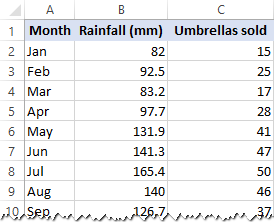
\includegraphics[width=0.7\linewidth]{accuracy/reg1.png}
%\end{figure}
%
%\pause
%
%Regression involves continuous data.
%\end{frame}

\begin{frame}{Metrics for Regression MSE \& MAE}
$$
\bordermatrix{&\text{Prediction}\;(\hat{y})\cr
               &10\cr
               &20\cr
                &30\cr
                &40\cr
               &50}
\qquad \qquad
\bordermatrix{&\text{Ground Truth}\;(y)\cr
               &20\cr
               &30\cr
                &40\cr
                &50\cr
               &60}
$$

\begin{align*}
\text{\textcolor{red}{Mean} \textcolor{green}{Squared} \textcolor{Tan}{Error} (MSE)} &=  \frac{\mathcolor{red}{\sum_{i=1}^{N}}(\mathcolor{Tan}{\hat{y}_i-y_i)}^{\mathcolor{green}2}}{\mathcolor{red}{N}} \\ 
\text{Root Mean Square Error (RMSE)} &=  \sqrt{\text{MSE}}
\end{align*}

\end{frame}

\begin{frame}{Accuracy Metrics: MAE \& ME}
$$
\bordermatrix{&\text{Prediction}\;(\hat{y})\cr
               &10\cr
               &20\cr
                &30\cr
                &40\cr
               &50}
\qquad \qquad
\bordermatrix{&\text{Ground Truth}\cr
               &20\cr
               &30\cr
                &40\cr
                &50\cr
               &60}
$$

\begin{align*}
\text{\textcolor{red}{Mean} \textcolor{green}{Absolute} \textcolor{Tan}{Error} (ME)} &=  \frac{\mathcolor{red}{\sum_{i=1}^{N}}\mathcolor{green}|\mathcolor{Tan}{\hat{y}_i-y_i\mathcolor{green}|}}{\mathcolor{red}{N}} \\ 
\text{Mean Error} &=  \frac{\sum_{i=1}^{N}\hat{y}_i-y_i}{N}
\end{align*}
\pause Is there any downside with using mean error?\\
\pause Errors can get cancelled out

\end{frame}


\begin{frame}{The Importance of Plotting}
\begin{figure}[htp]
    \centering
    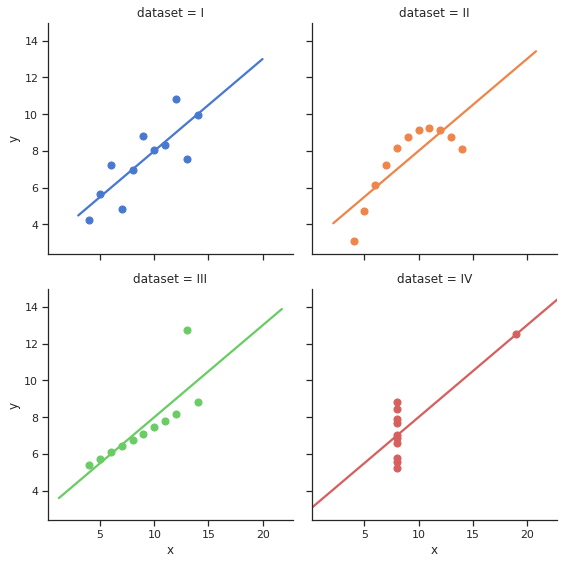
\includegraphics[width=0.6\linewidth]{ans1.png}
    \caption{Anscombe’s Quartet}
\end{figure}
\end{frame}

\begin{frame}{The Importance of Plotting}
\begin{tabular}{|c|c|c|}
\hline 
Property & Value & Accross datasets \\ 
\hline 
mean(X) & 9 & exact \\ 
mean(Y) & 7.5 & upto 3 decimal places \\ 
Linear regression line & 	y = 3.00 + 0.500x & upto 2 decimal places \\ 
\hline 
\end{tabular} 

Try to play with the \href{https://colab.research.google.com/drive/12Rrh7sf_lR-WUd4nYciOAKiil5kqWPAq}{colab link} to see how similar the metrics like variance and correlation are.

\end{frame}

\end{document}